\documentclass[12pt]{amsart}
\usepackage{amsmath, amssymb, amsthm}
\usepackage{geometry}
\usepackage{tikz}
\usepackage{graphicx}

\geometry{margin=1in}
\linespread{1.2}

\newtheorem{theorem}{Theorem}[section]
\newtheorem{question}[theorem]{Question}

\begin{document}
\begin{question}\label{ques:WLP-SLP}
For which graphs $G$ does the algebra $A(G)$ have the WLP or the SLP? When $A(G)$ fails to have one of these Lefschetz properties, in which degrees do the corresponding multiplication maps fail to have maximal rank?
\end{question}

The Lefschetz properties of $A(G)$ have been investigated in  for several classes of graphs, including complete graphs, star graphs, barbell graphs, wheel graphs, paths, cycles, and lollipop graphs. Artinian algebras defined by quadratic monomial relations have also been considered in earlier and recent works by Micha{\l}ek--Mir\'o-Roig , Migliore--Nagel--Schenck , Dao--Nair , Kling , Holleben , and Cooper et al. .

In the present paper, we instead focus on tadpole graphs. Recall that for integers $m \geq 3$ and $n \geq 1$, the {\it tadpole graph} $T_{m,n}$ is obtained by joining a cycle graph $C_m$ to a path graph $P_n$ by a bridge. More precisely, we label the vertices of $C_m$ by $x_1,\ldots,x_m$ and the vertices of $P_n$ by $y_1,\ldots,y_n$, and add the bridge $\{x_m,y_1\}$, see Figure~.

\begin{figure}[htbp]
\centering
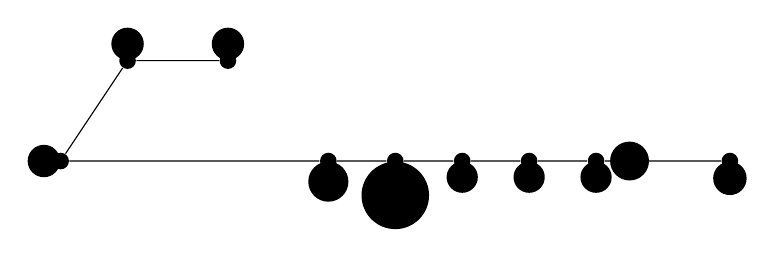
\begin{tikzpicture}[scale=0.85, every node/.style={circle, fill=black, inner sep=0pt, minimum size=6pt}]
    \node (x1) at (0,1.5) {};
    \node (x2) at (-1.5,1.5) {};
    \node (x3) at (-2.5,0) {};
    \node (xm) at (1.5,0) {};
    \node (ym) at (2.5,0) {};
    \node (y1) at (3.5,0) {};
    \node (y2) at (4.5,0) {};
    \node (y3) at (5.5,0) {};
    \node (yn) at (7.5,0) {};

    \draw (x1)--(x2)--(x3)--(xm)--(ym)--(y1)--(y2)--(y3)--(yn);

    \node[above] at (x1) {$x_1$};
    \node[above] at (x2) {$x_2$};
    \node[left] at (x3) {$x_3$};
    \node[below] at (xm) {$x_m$};
    \node[below] at (ym) {$x_{m-1}$};

    \node[below] at (y1) {$y_1$};
    \node[below] at (y2) {$y_2$};
    \node[below] at (y3) {$y_3$};
    \node[below] at (yn) {$y_n$};

    \node at (6,0) {$\cdots$};
\end{tikzpicture}
\caption{Tadpole $T_{m,n}$}
\label{fig:tadpole}
\end{figure}

Our main objective is to give a complete classification of the tadpole graphs $T_{m,n}$ for which the associated Artinian algebra $A(T_{m,n})$ has, or fails to have, the weak Lefschetz property. The classification is as follows.

\begin{theorem}\label{thm:main}
Assume that $\operatorname{char}(\Bbbk)=0$. The algebra $A(T_{m,n})$ has the weak Lefschetz property if and only if one of the following conditions holds:
\begin{enumerate}
\item[(i)] $m\in\{3,6,10\}$ and $n\in\{1,3,4,7\}$;
\item[(ii)] $m=4$ and $n\in\{1,2,\ldots,7,9,10,13\}$;
\item[(iii)] $m\in\{5,8\}$ and $n\in\{1,2,3,5,6,9\}$;
\item[(iv)] $m=7$ and $n\in\{1,2,3,4,7\}$;
\item[(v)] $(m,n)\in\{(9,1),(9,4),(11,2),(11,3),(11,6),(12,1),(13,1),(13,4),(14,3),(16,1)\}$.
\end{enumerate}
\end{theorem}

In addition to this classification, we study the independence polynomials of tadpole graphs. We prove that $I(T_{m,n};t)$ is unimodal for all $m\geq 3$ and $n\geq 1$, and we derive useful bounds for its mode. Recall that the independence polynomial of the path $P_n$ has mode $\lambda_n=\left\lceil\dfrac{5n+2-\sqrt{5n^2+20n+24}}{10}\right\rceil$.

\begin{theorem}\label{thm:unimodal}
The independence polynomial $I(T_{m,n};t)$ is unimodal for all $m\geq 3$ and $n\geq 1$. Moreover, for $m\geq 4$ and $n\geq 1$, its mode $\mu_{m,n}$ satisfies
$$
\lambda_{m-3}+\lambda_n-1\leq \mu_{m,n}\leq \lambda_{m-3}+\lambda_n+2.
$$
\end{theorem}
\end{document}
